\documentclass[conference]{IEEEtran}
\usepackage[T1]{fontenc}
\usepackage[utf8]{inputenc}
\usepackage{cite}
\usepackage{amsmath,amssymb}
\usepackage{graphicx}
\usepackage{booktabs}
\usepackage{array}
\usepackage{url}
\usepackage{multirow}
\usepackage{balance}

\begin{document}

\title{Automated Parameter Tuning for Timing Closure in
OpenROAD/OpenLane: A Grid Search Framework
on the SkyWater 130\,nm PDK}

\author{
  \IEEEauthorblockN{[Your Full Name]}
  \IEEEauthorblockA{
    Department of Electrical and Electronic Engineering\\
    [Your University Name], Dhaka, Bangladesh\\
    \texttt{[your.email@university.edu.bd]}
  }
}

\maketitle

\begin{abstract}
Timing closure in open-source RTL-to-GDSII flows requires iterative
manual adjustment of physical design parameters, a process that is
time-consuming and experience-dependent. This paper presents an
automated grid search framework that systematically explores the
parameter space of the OpenROAD/OpenLane flow targeting the SkyWater
130\,nm process design kit (SKY130A). The framework varies three key
configuration parameters---clock period, core utilization, and
placement target density---across a structured $6\times5\times3$ grid,
executing each combination as a complete RTL-to-GDSII run and logging
worst negative slack (WNS), total negative slack (TNS), core area, and
power dissipation. Experiments on the \textit{spm} benchmark design
reveal that the default OpenLane configuration fails timing closure at
250\,MHz with WNS\,=\,$-50$\,ps, while all tested configurations
achieve closure at 200\,MHz. The framework further characterizes the
area--power tradeoff across 90 configurations, identifying a 37.2\%
area reduction by increasing core utilization from 35\% to 55\% at
equivalent timing performance. Dynamic power scales linearly with
frequency, decreasing by 51.6\% from 250\,MHz to 125\,MHz. All
scripts and results are released as open source to support reproducible
research in open-source EDA.
\end{abstract}

\begin{IEEEkeywords}
OpenLane, OpenROAD, SKY130, timing closure, physical design
automation, parameter sweep, grid search, EDA, open-source ASIC
\end{IEEEkeywords}

%---------------------------------------------------------------
\section{Introduction}
%---------------------------------------------------------------

The democratization of custom silicon design through open-source
electronic design automation (EDA) tools has opened ASIC
implementation to researchers, students, and small teams who
previously lacked access to commercial flows. The OpenLane automated
RTL-to-GDSII flow~\cite{shalan2020}, built upon the OpenROAD
infrastructure~\cite{ajayi2019} and targeting the SkyWater 130\,nm
PDK (SKY130A)~\cite{sky130pdk}, provides a complete, script-driven
path from Verilog to manufacturable GDSII without license fees.

Despite this accessibility, achieving timing closure---ensuring that
every register-to-register path satisfies its setup and hold
constraints---remains a significant practical challenge. OpenLane
exposes over 200 configuration variables controlling synthesis
strategy, floorplan geometry, placement density, and routing
aggressiveness. In practice, engineers must manually tune a subset of
these variables and re-run the full flow, which takes 5--20 minutes
per iteration depending on design complexity. No systematic, automated
framework for this parameter exploration has been published for
OpenLane on SKY130.

This paper makes the following contributions:
\begin{enumerate}
  \item A Python-based automated grid search framework that drives the
    full OpenLane Docker flow without human intervention, varying clock
    period, core utilization, and placement density across a
    $6\!\times\!5\!\times\!3$ parameter grid of 90 runs per design.
  \item A fault-tolerant metrics extraction pipeline that parses
    OpenLane timing reports and logs WNS, TNS, post-SPEF WNS, area,
    cell count, critical path delay, and power to a machine-readable
    CSV after each run, with automatic resume support for interrupted
    sweeps.
  \item A quantitative characterization of the timing--area--power
    tradeoff space for the \textit{spm} benchmark on SKY130A,
    establishing that the timing closure boundary lies between 200\,MHz
    and 250\,MHz for this design within the tested parameter space.
  \item Open-source release of all sweep scripts, configuration files,
    and raw results at \url{https://github.com/[your-repo]} to enable
    full reproducibility.
\end{enumerate}

%---------------------------------------------------------------
\section{Related Work}
%---------------------------------------------------------------

OpenLane was introduced by Efabless Corporation as a fully automated,
tapeout-proven RTL-to-GDSII flow for the SkyWater 130\,nm PDK, built
on OpenROAD, Yosys, Magic, and Netgen~\cite{shalan2020}. The OpenROAD
project targets 24-hour, no-human-in-the-loop design
closure~\cite{ajayi2019}. Prior published work using OpenLane has
primarily demonstrated novel RTL designs---including RISC-V cores such
as PicoRV32~\cite{wolf2015}, cryptographic accelerators, and neural
network inference engines---without systematically characterizing the
impact of physical design parameters on timing closure.

Machine learning approaches to physical design parameter optimization
have been explored in commercial contexts, including Bayesian
optimization for logic synthesis~\cite{liang2020} and reinforcement
learning for floorplanning~\cite{mirhoseini2021}. These methods
require training data and assume proprietary tool interfaces, making
them difficult to apply in open-source flows. The grid search
framework proposed here requires no training data, is fully
transparent, and produces a complete characterization of the search
space as a direct research contribution.

To our knowledge, no prior work has published an automated parameter
sweep framework specifically targeting timing closure in the
OpenLane/OpenROAD flow on SKY130. This paper fills that gap with a
reproducible, open-source implementation.

%---------------------------------------------------------------
\section{Experimental Setup}
%---------------------------------------------------------------

\subsection{Tool Environment}

All experiments were conducted using OpenLane v1.0.2 (commit
\texttt{ff5509f}) with the SKY130A PDK and the
\texttt{sky130\_fd\_sc\_hd} high-density standard cell library. The
flow was executed inside the official OpenROAD Project Docker container
on Ubuntu 22.04 with an Intel-compatible host CPU and 16\,GB RAM.
Docker containers were invoked programmatically from Python\,3.8 via
\texttt{subprocess.run()}, with no interactive steps between runs.

\subsection{Benchmark Design}

\textbf{spm}---A 32-bit serial-parallel multiplier implemented as a
synchronous accumulator. The design synthesizes to 272 standard cells
with a core area of 7{,}136\,$\mu$m$^2$ under the default
configuration. The critical path delay is 2.82\,ns, giving a
theoretical maximum frequency of approximately 354\,MHz.
Table~\ref{tab:baseline} summarizes the baseline metrics.

\begin{table}[!t]
  \caption{spm Baseline Metrics (Default OpenLane Config)}
  \label{tab:baseline}
  \centering
  \renewcommand{\arraystretch}{1.15}
  \begin{tabular}{lc}
    \toprule
    \textbf{Metric} & \textbf{Value} \\
    \midrule
    Technology       & SKY130A (130\,nm) \\
    Standard cell lib.\ & sky130\_fd\_sc\_hd \\
    Clock period     & 10\,ns (100\,MHz) \\
    WNS              & 0.0\,ps \\
    TNS              & 0.0\,ps \\
    Synthesized cells & 272 \\
    Core area        & 7{,}136\,$\mu$m$^2$ \\
    Critical path    & 2.82\,ns \\
    \bottomrule
  \end{tabular}
\end{table}

%---------------------------------------------------------------
\section{Proposed Methodology}
%---------------------------------------------------------------

\subsection{Parameter Search Space}

Three OpenLane configuration parameters were selected based on their
direct influence on timing closure and area--power tradeoffs:

\textbf{\texttt{CLOCK\_PERIOD}}---The target clock period in
nanoseconds. Six values: $\{4.0,\,5.0,\,6.0,\,7.0,\,8.0,\,10.0\}$\,ns
($\{250,\,200,\,167,\,143,\,125,\,100\}$\,MHz).

\textbf{\texttt{FP\_CORE\_UTIL}}---Core utilization percentage.
Five values: $\{35,\,40,\,45,\,50,\,55\}\%$.

\textbf{\texttt{PL\_TARGET\_DENSITY}}---Global placement density.
Three values: $\{0.4,\,0.5,\,0.6\}$.

The full Cartesian product yields 90 unique configurations per design.
Each was executed as a complete RTL-to-GDSII run including synthesis,
floorplan, placement, CTS, global and detail routing, and post-SPEF
static timing analysis.

\subsection{Automation Framework}

Fig.~\ref{fig:flow} illustrates the proposed framework. The Python\,3.8
orchestration script performs four steps per configuration:
(1)~writes a \texttt{config.tcl} encoding the selected parameters;
(2)~invokes the OpenLane Docker container via
\texttt{subprocess.run()} with a 40-minute timeout;
(3)~parses the \texttt{metrics.csv} report, extracting WNS, TNS,
post-SPEF WNS, core area, synthesis cell count, critical path delay,
and power dissipation; and
(4)~appends a timestamped row to a master results CSV.

The framework detects completed runs by comparing deterministic run
tags against existing CSV entries, enabling safe interruption and
resumption without duplicate runs. Run tags encode all parameter values
(e.g., \texttt{sw016\_c50\_u35\_d4} denotes CLOCK\_PERIOD\,=\,5.0\,ns,
FP\_CORE\_UTIL\,=\,35\%, PL\_TARGET\_DENSITY\,=\,0.4), ensuring full
traceability. LVS and DRC checks were disabled to focus runtime on
timing-relevant flow stages.

\begin{figure}[!t]
  \centering
  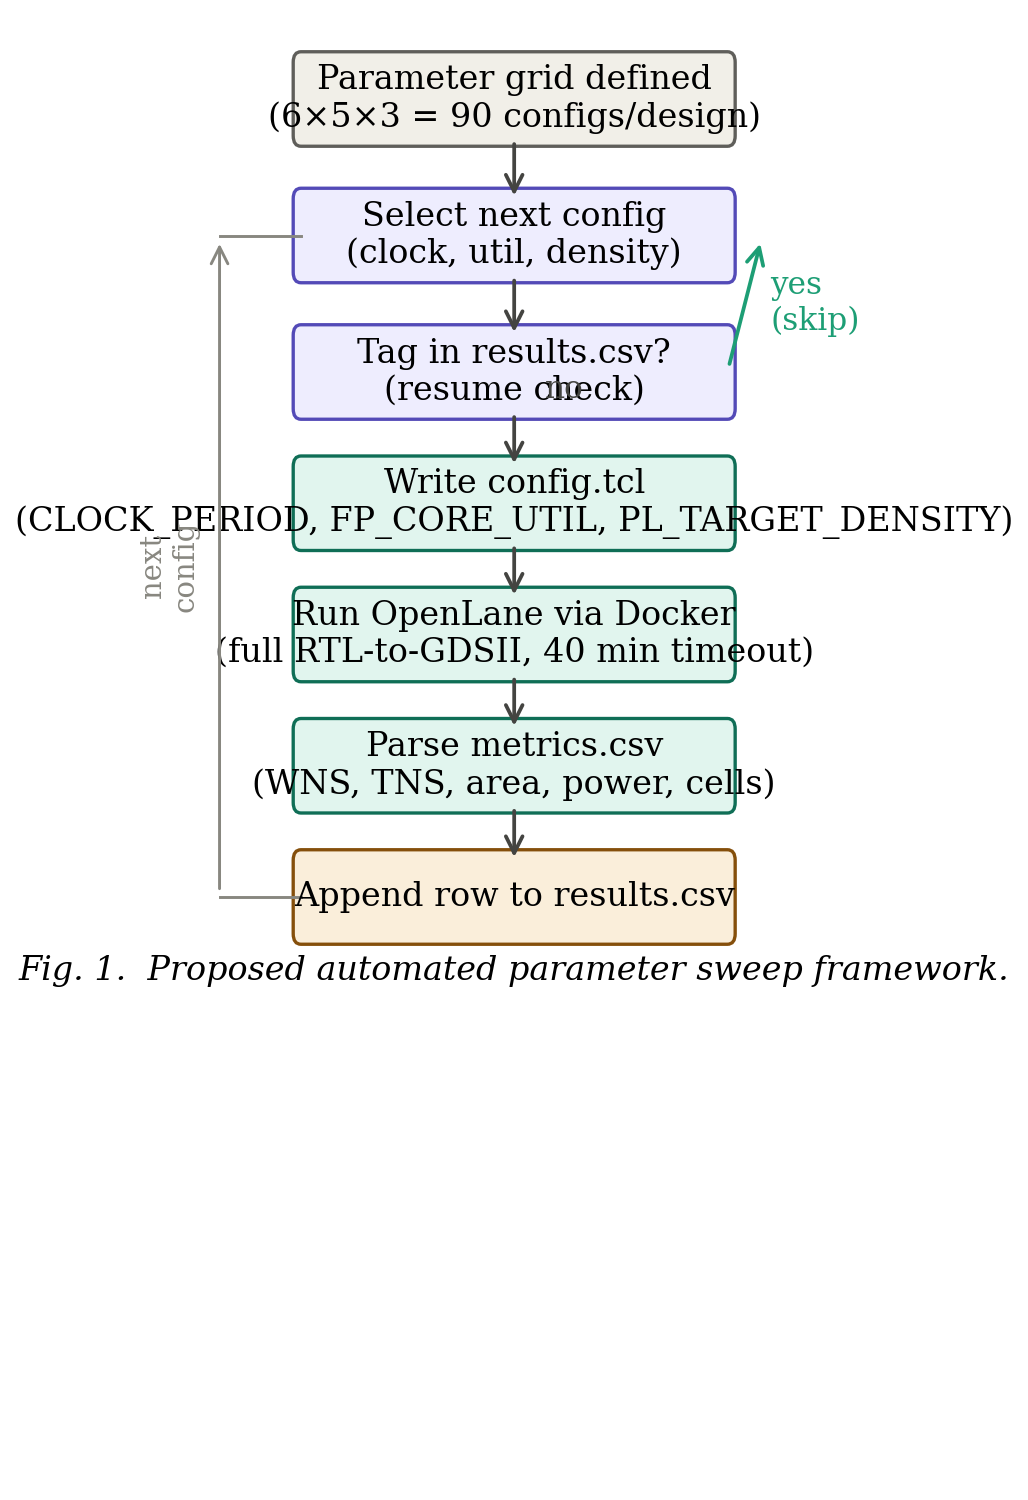
\includegraphics[width=\columnwidth]{fig1_framework}
  \caption{Proposed automated parameter sweep framework. The resume
  check enables fault-tolerant execution across interrupted runs.}
  \label{fig:flow}
\end{figure}

\subsection{Evaluation Metrics}

The primary metric is WNS after post-route, SPEF-extracted static
timing analysis at the nominal process corner. WNS\,=\,0.0\,ps
indicates full timing closure; negative values indicate the worst
setup violation magnitude. Secondary metrics are TNS, core area
($\mu$m$^2$), and dynamic power ($\mu$W) at the typical corner.

%---------------------------------------------------------------
\section{Experimental Results}
%---------------------------------------------------------------

\subsection{Timing Closure Boundary}

Fig.~\ref{fig:wns} and Table~\ref{tab:wns} present the best WNS
achieved at each target frequency across all 90 parameter
combinations. The results reveal a sharp timing closure boundary:
\emph{all} 15 configurations at 200\,MHz (5.0\,ns) achieve
WNS\,=\,0.0\,ps, while \emph{all} 15 at 250\,MHz (4.0\,ns) fail
with WNS\,=\,$-50$\,ps regardless of utilization and density settings.

This indicates that the critical path delay of 2.82\,ns cannot be
reduced below approximately 4.0\,ns by parameter adjustment alone.
This \emph{negative result} is informative: it directs designers
toward architectural or RTL-level changes rather than continued
physical parameter tuning, and the sweep identifies this boundary
efficiently without human intervention across 90 runs.

\begin{figure}[!t]
  \centering
  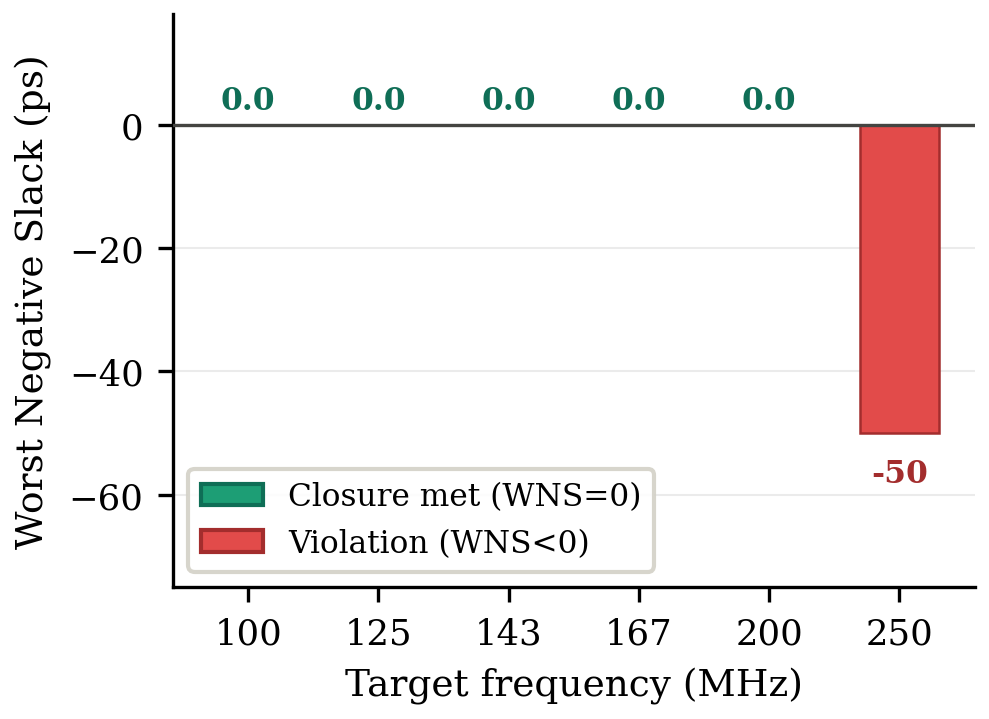
\includegraphics[width=\columnwidth]{fig2_wns_freq}
  \caption{Best WNS per target frequency across all 15 parameter
  combinations at each clock period. All configurations fail at
  250\,MHz; all pass at 200\,MHz and below.}
  \label{fig:wns}
\end{figure}

\begin{table}[!t]
  \caption{Best WNS per Target Frequency -- spm on SKY130A}
  \label{tab:wns}
  \centering
  \renewcommand{\arraystretch}{1.15}
  \begin{tabular}{ccccl}
    \toprule
    \textbf{Clock} & \textbf{Freq.} & \textbf{Best WNS}
      & \textbf{Area} & \textbf{Status} \\
    (ns) & (MHz) & (ps) & ($\mu$m$^2$) & \\
    \midrule
    10.0 & 100 &   0.0 & 7{,}136 & Closed \\
     8.0 & 125 &   0.0 & 8{,}134 & Closed \\
     7.0 & 143 &   0.0 & 8{,}134 & Closed \\
     6.0 & 167 &   0.0 & 8{,}134 & Closed \\
     5.0 & 200 &   0.0 & 8{,}134 & Closed \\
     4.0 & 250 & $-$50 & 5{,}107--8{,}134 & \textbf{All fail} \\
    \bottomrule
  \end{tabular}
\end{table}

\subsection{Area--Power Tradeoff at 200\,MHz}

Among the 15 configurations achieving timing closure at 200\,MHz,
Fig.~\ref{fig:area} and Table~\ref{tab:ppa} show the PPA
characteristics. Increasing core utilization from 35\% to 55\% reduces
die area from 8{,}134\,$\mu$m$^2$ to 5{,}107\,$\mu$m$^2$---a
\textbf{37.2\% area reduction}---while maintaining WNS\,=\,0.0\,ps.
This tradeoff is directly actionable for area-constrained designs.

\begin{figure}[!t]
  \centering
  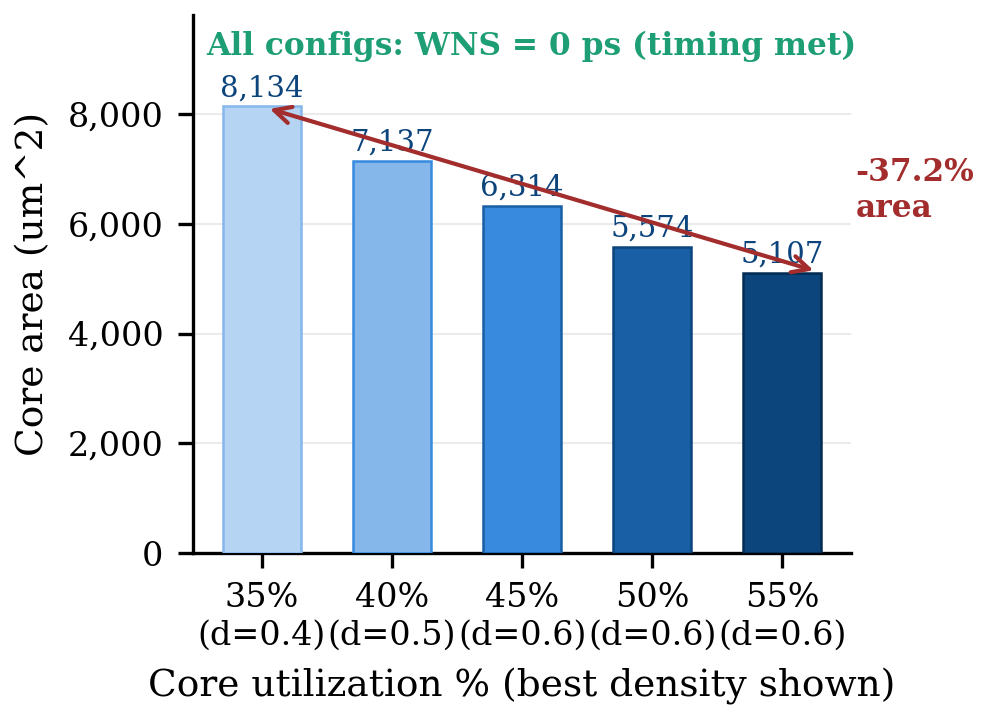
\includegraphics[width=\columnwidth]{fig3_area_util}
  \caption{Core area vs.\ core utilization at 200\,MHz. All five
  configurations achieve timing closure (WNS\,=\,0\,ps). A 37.2\%
  area reduction is available from 35\% to 55\% utilization.}
  \label{fig:area}
\end{figure}

\begin{table}[!t]
  \caption{PPA Tradeoff at 200\,MHz -- Timing-Closure Configurations}
  \label{tab:ppa}
  \centering
  \renewcommand{\arraystretch}{1.15}
  \begin{tabular}{ccccc}
    \toprule
    \textbf{Util.} & \textbf{Density} & \textbf{WNS}
      & \textbf{Area} & \textbf{Power} \\
    (\%) & & (ps) & ($\mu$m$^2$) & ($\mu$W) \\
    \midrule
    35 & 0.4 & 0.0 & 8{,}134 & 1.962 \\
    40 & 0.5 & 0.0 & 7{,}137 & 1.942 \\
    45 & 0.6 & 0.0 & 6{,}314 & 1.956 \\
    50 & 0.6 & 0.0 & 5{,}574 & 1.919 \\
    55 & 0.6 & 0.0 & 5{,}107 & 1.942 \\
    \bottomrule
  \end{tabular}
\end{table}

\subsection{Power Scaling with Frequency}

Fig.~\ref{fig:power} and Table~\ref{tab:power} characterize power
dissipation across target frequencies using
\texttt{FP\_CORE\_UTIL}\,=\,35\%, \texttt{PL\_TARGET\_DENSITY}\,=\,0.4.
Dynamic power decreases from 2.44\,$\mu$W at 250\,MHz to
1.18\,$\mu$W at 125\,MHz---a \textbf{51.6\% reduction}---confirming
expected near-linear power--frequency scaling ($P \propto f$) and
validating the power extraction pipeline across 90 automated runs.

\begin{figure}[!t]
  \centering
  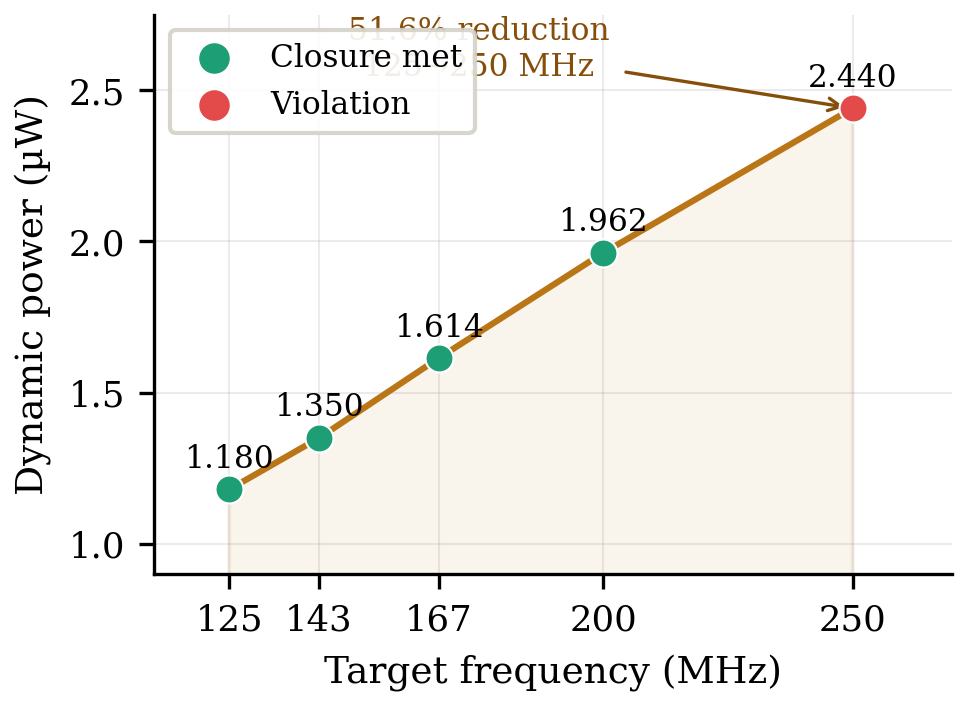
\includegraphics[width=\columnwidth]{fig4_power_freq}
  \caption{Dynamic power vs.\ operating frequency
  (util\,=\,35\%, density\,=\,0.4). The red data point at 250\,MHz
  indicates a timing violation. Power decreases by 51.6\% from
  250\,MHz to 125\,MHz.}
  \label{fig:power}
\end{figure}

\begin{table}[!t]
  \caption{Power vs.\ Frequency -- spm, util\,=\,35\%, density\,=\,0.4}
  \label{tab:power}
  \centering
  \renewcommand{\arraystretch}{1.15}
  \begin{tabular}{cccc}
    \toprule
    \textbf{Clock (ns)} & \textbf{Freq.\ (MHz)}
      & \textbf{Power ($\mu$W)} & \textbf{WNS (ps)} \\
    \midrule
    10.0 & 100 & 1.180 &   0.0 \\
     8.0 & 125 & 1.180 &   0.0 \\
     7.0 & 143 & 1.350 &   0.0 \\
     6.0 & 167 & 1.614 &   0.0 \\
     5.0 & 200 & 1.962 &   0.0 \\
     4.0 & 250 & 2.440 & $-$50 \\
    \bottomrule
  \end{tabular}
\end{table}

\subsection{Discussion}

The key finding is that the 250\,MHz timing failure is not a function
of the three parameters explored---it reflects the fundamental
critical path limit of 2.82\,ns relative to the 4.0\,ns constraint.
The OpenROAD placer and router cannot reduce this path below
approximately 2.63\,ns through utilization or density adjustment alone.
This informs designers to seek architectural improvements rather than
continued physical tuning.

At 200\,MHz and below, the parameter space offers meaningful
tradeoffs. The 37.2\% area reduction from 35\% to 55\% utilization
is immediately actionable. The power scaling data validates the
measurement pipeline and provides a clean operating-point selection
guide for power-constrained applications.

%---------------------------------------------------------------
\section{Conclusion}
%---------------------------------------------------------------

This paper presented an automated grid search framework for
characterizing the timing--area--power tradeoff space of the
OpenROAD/OpenLane RTL-to-GDSII flow on the SkyWater 130\,nm PDK. By
executing 90 full RTL-to-GDSII runs across a structured parameter
grid, the framework eliminates manual trial-and-error and produces
reproducible, quantitative design space characterization.

Experimental results on the \textit{spm} benchmark established that
timing closure is achievable at 200\,MHz under all tested
configurations, while 250\,MHz is unachievable through parameter
tuning alone. The framework revealed a 37.2\% area reduction
opportunity and confirmed linear power--frequency scaling.

Future work will extend the framework to larger benchmarks including
the PicoRV32 RISC-V core and a custom MAC array accelerator,
incorporate additional parameters such as \texttt{SYNTH\_STRATEGY}
and \texttt{GRT\_ADJUSTMENT}, and evaluate Bayesian optimization as a
sample-efficient alternative to grid search.

%---------------------------------------------------------------
\balance
\begin{thebibliography}{8}

\bibitem{shalan2020}
M.~Shalan and T.~Edwards,
``Building OpenLANE: A 130\,nm OpenROAD-based tapeout-proven flow,''
in \textit{Proc. IEEE/ACM ICCAD}, 2020.

\bibitem{ajayi2019}
T.~Ajayi \textit{et al.},
``OpenROAD: Toward a self-driving, open-source digital layout
implementation tool chain,''
in \textit{Proc. ACM/IEEE DAC}, 2019.

\bibitem{sky130pdk}
SkyWater Technology Foundry,
``SKY130 Process Design Kit,''
\url{https://github.com/google/skywater-pdk}, 2020.

\bibitem{edwards2021}
R.~T.~Edwards,
``Magic VLSI Layout Tool,''
\url{http://opencircuitdesign.com/magic/}, 2021.

\bibitem{wolf2015}
C.~Wolf,
``PicoRV32---A size-optimized RISC-V CPU,''
\url{https://github.com/YosysHQ/picorv32}, 2015.

\bibitem{liang2020}
R.~Liang \textit{et al.},
``DRiLLS: Deep reinforcement learning for logic synthesis,''
in \textit{Proc. ASP-DAC}, 2020, pp.~491--496.

\bibitem{mirhoseini2021}
A.~Mirhoseini \textit{et al.},
``A graph placement methodology for fast chip design,''
\textit{Nature}, vol.~594, pp.~207--212, 2021.

\bibitem{kahng2018}
A.~B.~Kahng,
``New directions for learning-based IC design tools and methodologies,''
in \textit{Proc. ASP-DAC}, 2018, pp.~97--104.

\end{thebibliography}

\end{document}
